% Task 5 — Regional Hub Selection and Network Definition
% Northeast Megaregion Freight Network Design
% All throughput figures are in thousand short tons (ktons); distances in miles; capacity in square feet (sf).

\section{Task 5 — Regional Hub Selection and Network Design}

Task 5 selects one regional hub per logistics region and defines the topology of the
regional hub network. Hub selection is formulated as a capacity-aware set-cover Mixed
Integer Program (MIP) solved over the 1,862-candidate Task~4 pool; network link
definition uses a hybrid flow-weighted refinement of Delaunay triangulation.

\subsection{Candidate Pre-Processing: Set $H$ and Feasibility Set $Z$}

\paragraph{Road-accessibility gate.}
Before the MIP is built, each candidate in the primary pool is attributed with its
Euclidean distance $d_h^{\text{road}}$ to the nearest US interstate segment (NTAD
North American Roads, \texttt{CLASS=1}, \texttt{COUNTRY=2}, projected to EPSG:9311
via a spatial STRtree index). The 90th-percentile distance $\beta = 12{,}831$~m
(approximately 8.0~miles) is used as a hard gate: the 187 candidates exceeding this
threshold are excluded from the active candidate set $H$, leaving $|H| = 1{,}675$
facilities. Among the 50 selected hubs, road proximity ranges from 0.13 to 7.79~miles
(mean 1.71~miles, median 1.11~miles), confirming strong interstate access across the
final set.

\paragraph{Feasibility set $Z$.}
All hub–region pairs $(h, r)$ within a Euclidean radius of 150~miles
($241{,}402$~m, EPSG:9311) form the feasibility set $Z$. This yields
$|Z| = 26{,}133$ feasible pairs; every one of the 50 regions has at least one
feasible candidate, including region~25, which has no in-region candidate after
$\beta$-gating but is covered by 708 external candidates within the 150-mile radius.

\subsection{MIP Formulation}

\paragraph{Sets, parameters, and variables.}

Let $H$ be the road-gated candidate set, $R$ the 50 Task~3 regions, and
$Z \subseteq H \times R$ the feasibility set. The key parameters are:

\begin{itemize}
  \item $s_h$ — usable available floor area of hub $h$ (sf), from Task~4;
  \item $w_{cr}$ — 2025 external throughput of county $c$ in region $r$ (ktons),
        as the demand weight;
  \item $d_{hcr}$ — Euclidean distance from hub $h$ to county centroid $c$ in region $r$;
  \item $\bar{Q} = 306{,}250$~sf — median $s_h$ across $H$, used as a neutral capacity
        reference;
  \item $T_r$ — total 2025 external throughput of region $r$; $\bar{T}$ — mean over all
        50 regions.
\end{itemize}

The per-assignment cost coefficient incorporates a square-root capacity discount:

\begin{equation}
  \hat{c}_{hr} = \left(\sum_{c \in C_r} w_{cr} \cdot d_{hcr}\right)
    \cdot \left(\frac{\bar{Q}}{s_h}\right)^{0.5}
  \label{eq:task5-cost}
\end{equation}

This formulation keeps geography the primary driver while giving larger facilities a
moderate cost reduction: a facility at the capacity cap (500k~sf) receives approximately
a 37\% discount relative to the minimum qualifying facility (200k~sf).

Binary variables $A_{hr} \in \{0,1\}$ indicate assignment of hub $h$ to serve region
$r$; $O_h \in \{0,1\}$ indicates whether hub $h$ is opened.

\paragraph{Objective and constraints.}

\begin{equation}
  \min \sum_{(h,r) \in Z} A_{hr} \cdot \hat{c}_{hr}
  \label{eq:task5-obj}
\end{equation}

\begin{align}
  \sum_{h:\,(h,r)\in Z} A_{hr} &\geq 1
    && \forall r \in R
    & \text{(coverage)} \label{eq:t5-cov} \\[4pt]
  \sum_{r:\,(h,r)\in Z} A_{hr} &\leq 2
    && \forall h \in H
    & \text{(concentration cap)} \label{eq:t5-cap} \\[4pt]
  O_h &\leq \sum_{r:\,(h,r)\in Z} A_{hr}
    && \forall h \in H
    & \text{(activation)} \label{eq:t5-act} \\[4pt]
  \sum_{h:\,(h,r)\in Z} A_{hr} \cdot s_h &\geq \bar{Q} \cdot \frac{T_r}{\bar{T}}
    && \forall r \in R
    & \text{(capacity)} \label{eq:t5-capcov} \\[4pt]
  A_{hr},\, O_h &\in \{0,1\}
    &&& \label{eq:t5-bin}
\end{align}

Constraint~\eqref{eq:t5-cov} ensures every region receives at least one hub.
Constraint~\eqref{eq:t5-cap} limits each hub to serving at most two regions,
preventing over-concentration. Constraint~\eqref{eq:t5-capcov} scales the required
assigned floor area proportionally to each region's freight demand: high-demand regions
must attract larger or multiple hubs.

\subsection{Solution and Hub Characterization}

Gurobi finds the \textbf{optimal} solution in 0.14~s at a 0.44\% MIP gap.
Table~\ref{tab:task5-results} summarises the outcome.

\begin{table}[H]
  \centering
  \caption{Task 5 MIP solution summary.}
  \label{tab:task5-results}
  \begin{tabular}{lr}
    \toprule
    Metric & Value \\
    \midrule
    Selected regional hubs & 50 \\
    Hub-region assignments & 52 \\
    Hubs serving 1 region & 48 \\
    Hubs serving 2 regions & 2 \\
    Solve time & 0.14~s \\
    MIP gap & 0.44\% \\
    Solver status & Optimal \\
    \midrule
    Median hub capacity & 449{,}340~sf \\
    Mean hub capacity & 435{,}339~sf \\
    Min / max hub capacity & 285{,}146 / 500{,}000~sf \\
    Median road distance & 1.11~miles \\
    \bottomrule
  \end{tabular}
\end{table}

All 50 regions achieve coverage. Two hubs serve dual regions to satisfy demand-scaled
capacity constraints: one hub covers regions~34 and~45, and a second covers
regions~4 and~41 — both pairs are geographically proximate, so the dual assignment
remains operationally coherent. Four hubs are assigned to serve a region other than
their own home region, indicating that the optimizer occasionally selects a high-capacity
cross-boundary facility when the in-region pool lacks sufficient floor area at
acceptable distance.

Table~\ref{tab:task5-state} shows the state distribution of selected hubs, which
broadly mirrors the distribution of logistics infrastructure in the megaregion.
Pennsylvania leads with 14 hubs, consistent with its role as the primary inland
distribution corridor.

\begin{table}[H]
  \centering
  \caption{Regional hub count by state.}
  \label{tab:task5-state}
  \begin{tabular}{lr}
    \toprule
    State & Selected hubs \\
    \midrule
    PA & 14 \\
    VA & 11 \\
    NY & \phantom{0}8 \\
    NJ & \phantom{0}7 \\
    MD & \phantom{0}3 \\
    CT & \phantom{0}2 \\
    DE & \phantom{0}1 \\
    MA & \phantom{0}1 \\
    ME & \phantom{0}1 \\
    RI & \phantom{0}1 \\
    WV & \phantom{0}1 \\
    \midrule
    \textbf{Total} & \textbf{50} \\
    \bottomrule
  \end{tabular}
\end{table}

Figure~\ref{fig:task5-hubs} shows the geographic distribution of selected regional hubs.

\begin{figure}[H]
  \centering
  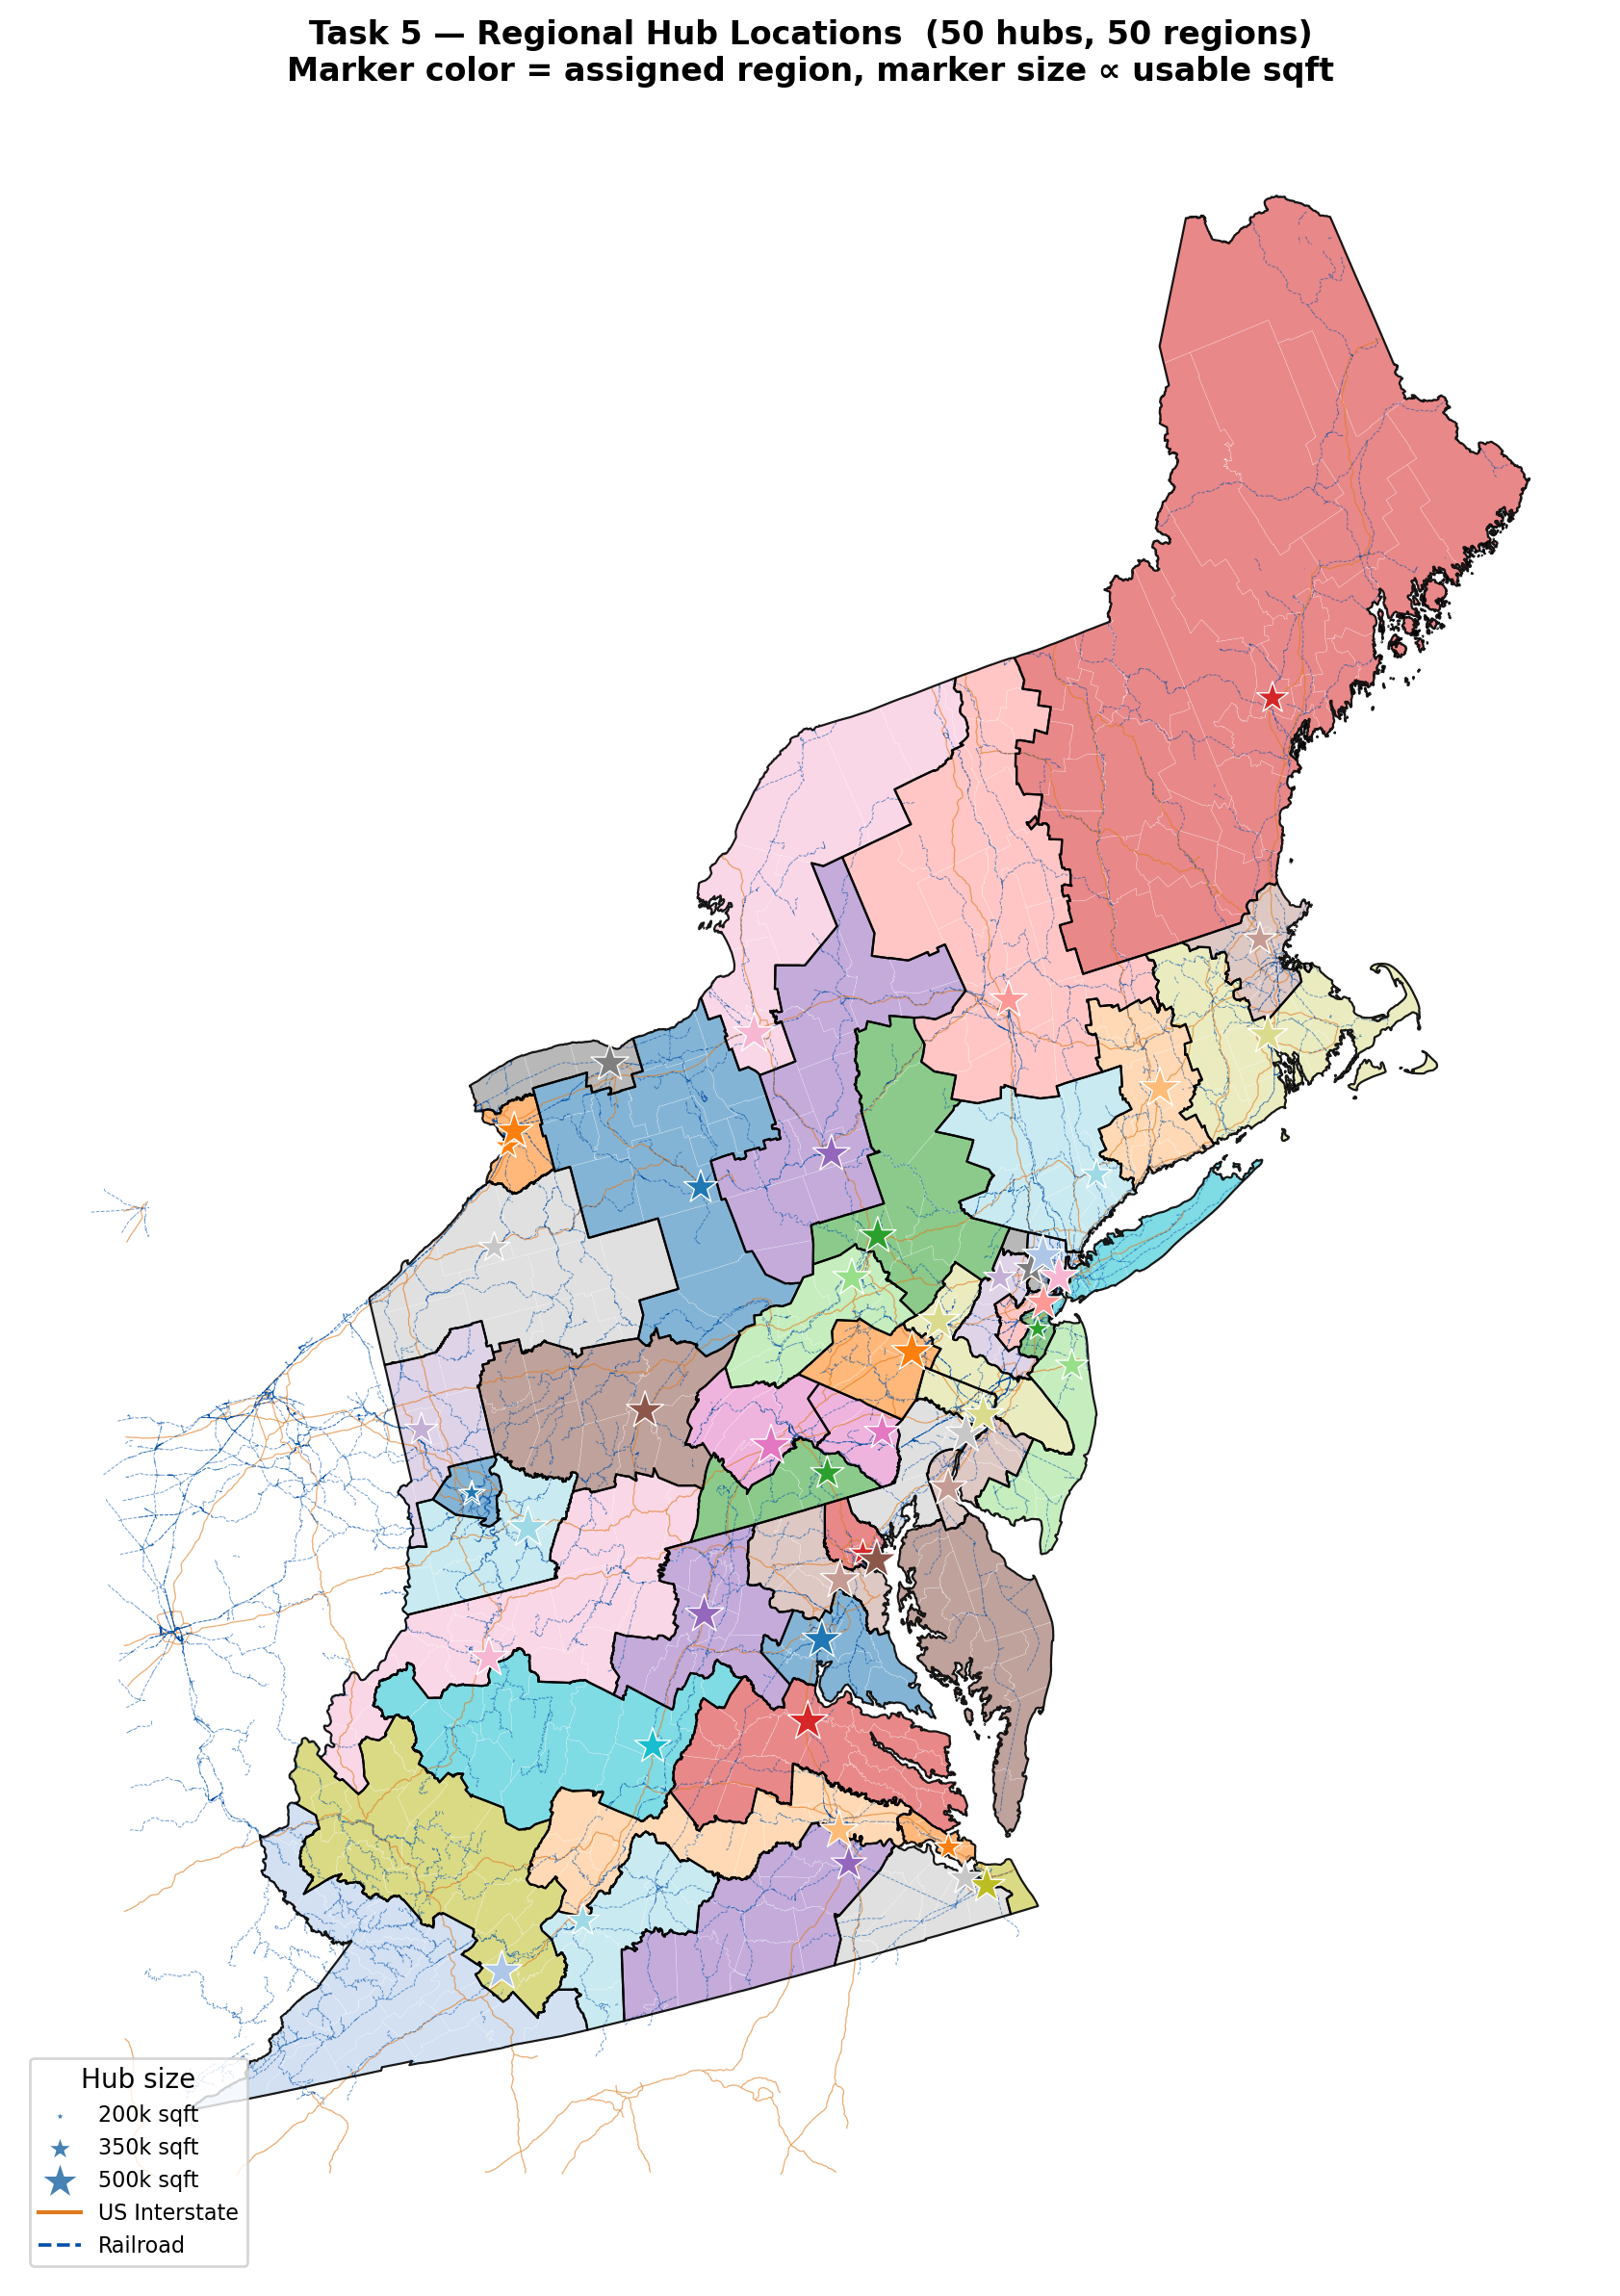
\includegraphics[width=0.90\textwidth]{figures/task5_hub_locations.png}
  \caption{Selected regional hubs across the 14-state Northeast megaregion. Marker size
    is proportional to usable available floor area; colour indicates the assigned
    Task~3 region. The heavy concentration in the PA--NJ--VA corridor reflects both
    logistics density and the demand-weighted geographic cost minimised by the MIP.}
  \label{fig:task5-hubs}
\end{figure}

\subsection{Flow-Weighted Network Topology}

\paragraph{Hybrid link definition.}
The regional hub network is built in three stages. First, a Delaunay triangulation over
the 50 hub locations provides a spatially connected baseline; links exceeding 350~miles
are pruned, yielding 137 candidate links. Second, a region-to-region freight interaction
matrix is computed from the Task~1 truck-compatible O-D flows (excluding SCTG coal and
gravel), aggregated to 50$\times$50 region pairs. Third, a hybrid refinement is applied:

\begin{itemize}
  \item \textbf{Prune}: remove links where flow intensity falls below the 10th percentile
        ($< 1{,}001$~ktons) \emph{and} distance exceeds the 70th percentile
        ($> 93$~miles) — 9 links removed.
  \item \textbf{Supplement}: add links where flow intensity is at or above the 75th
        percentile ($\geq 8{,}787$~ktons) \emph{and} distance is $\leq 350$~miles, if
        not already present — 5 links added.
\end{itemize}

The final network contains \textbf{133 links}. Table~\ref{tab:task5-network} compares
the Delaunay baseline to the flow-weighted result.

\begin{table}[H]
  \centering
  \caption{Regional hub network comparison: Delaunay baseline vs.\ flow-weighted final.}
  \label{tab:task5-network}
  \begin{tabular}{lrr}
    \toprule
    Metric & Delaunay (137 links) & Flow-weighted (133 links) \\
    \midrule
    Mean flow intensity (ktons) & 6{,}912 & 7{,}532 \\
    Min flow intensity (ktons) & \phantom{0,0}92 & \phantom{0,0}516 \\
    Mean distance (miles) & 75.9 & 69.2 \\
    Max distance (miles) & — & 305.6 \\
    \bottomrule
  \end{tabular}
\end{table}

The hybrid refinement increases mean flow intensity by 9\% and raises the minimum from
92 to 516~ktons — eliminating marginal low-volume, long-distance links while preserving
or adding high-volume corridors. Mean link distance falls by 8.8~miles, reflecting the
removal of geographically inefficient connections such as the Howell~NJ to
Chesapeake~VA link (261~miles, 92~ktons) and the addition of shorter high-volume
corridors (e.g., Buffalo Road to the FedEx hub, 65~miles, 15{,}280~ktons).

Figure~\ref{fig:task5-network} shows the flow-weighted network with link thickness
proportional to freight interaction intensity.

\begin{figure}[H]
  \centering
  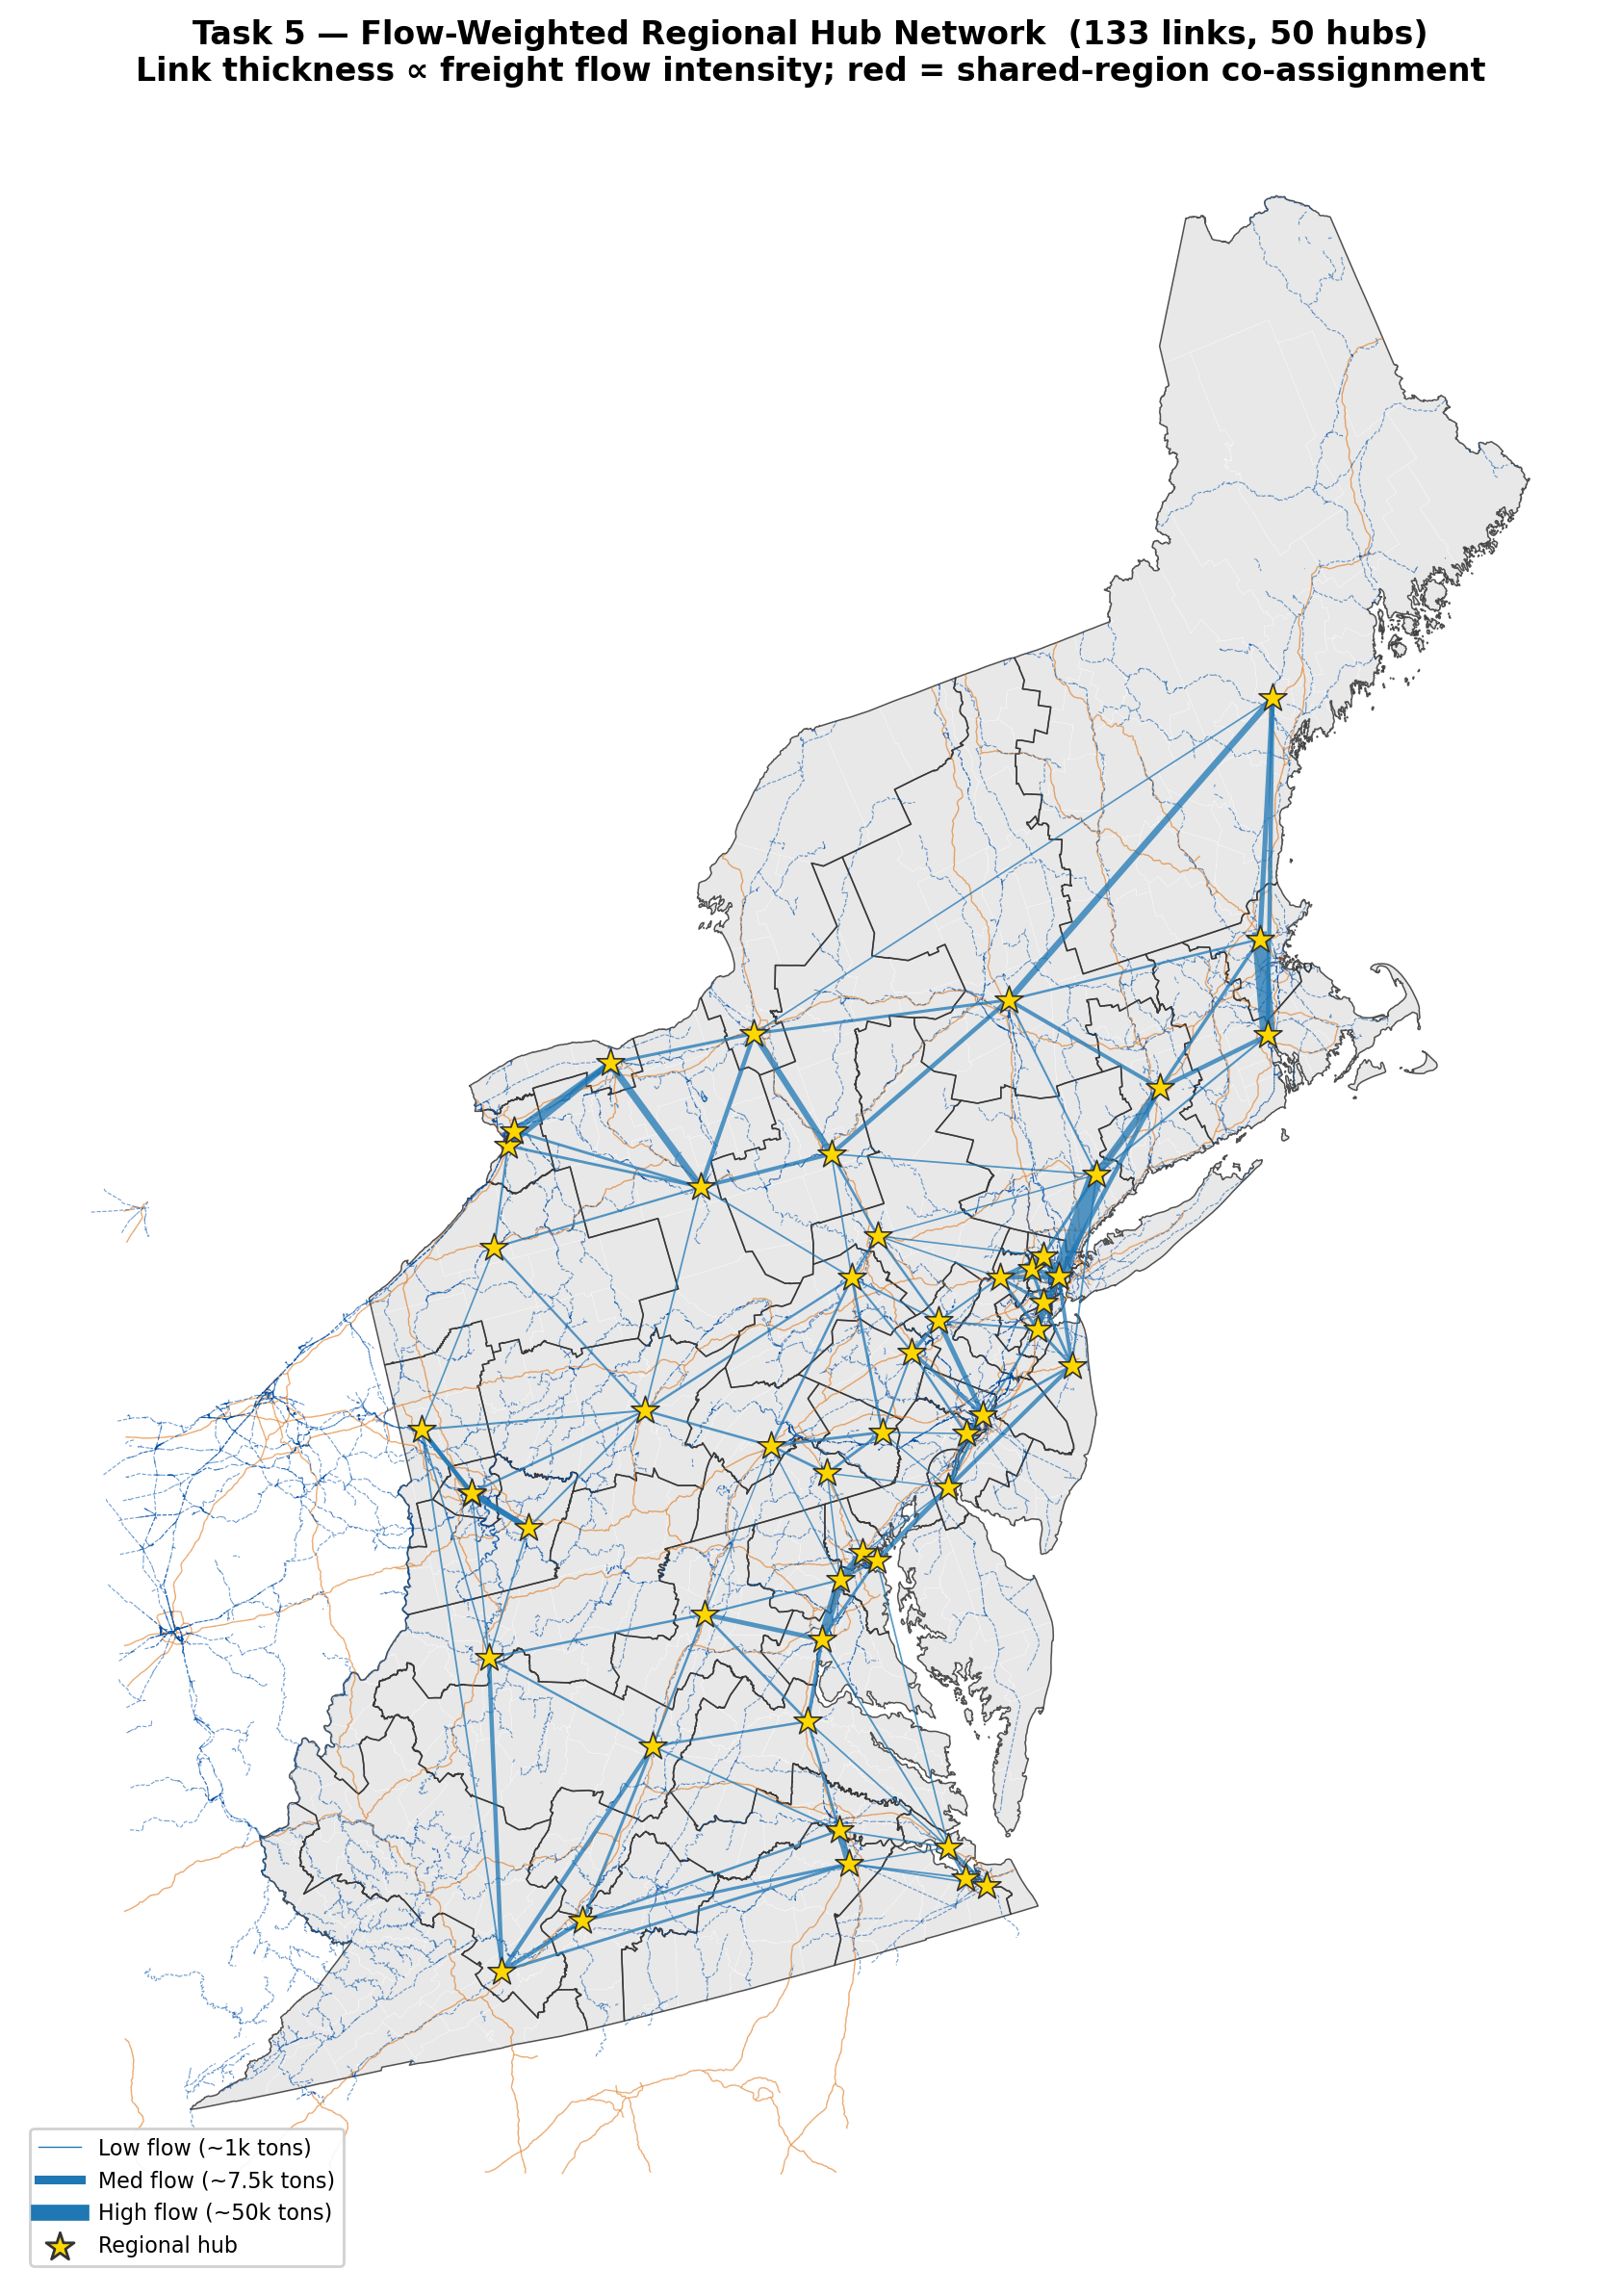
\includegraphics[width=0.90\textwidth]{figures/task5_hub_network.png}
  \caption{Flow-weighted regional hub network (133 links). Link thickness is proportional
    to freight flow intensity (range: 516--51{,}469~ktons). Thicker links concentrate
    along the I-95 coastal belt and the PA--NY axis, consistent with the high-intensity
    freight corridors identified in Task~1.}
  \label{fig:task5-network}
\end{figure}

The maximum link drive time is 4.78~h and the mean is 1.08~h, keeping the inter-hub
network well within the 5.5-hour operational constraint. All 50 hubs participate in the
connected network, providing redundant routing paths that support the multi-tier
consolidation logic defined in downstream tasks.
